% ==================================================================================================
\subsection{Homogenizing Effect of Turnover}\label{aa:homogenize}
% TODO: update this figure
\begin{figure}[H]
  \centering
  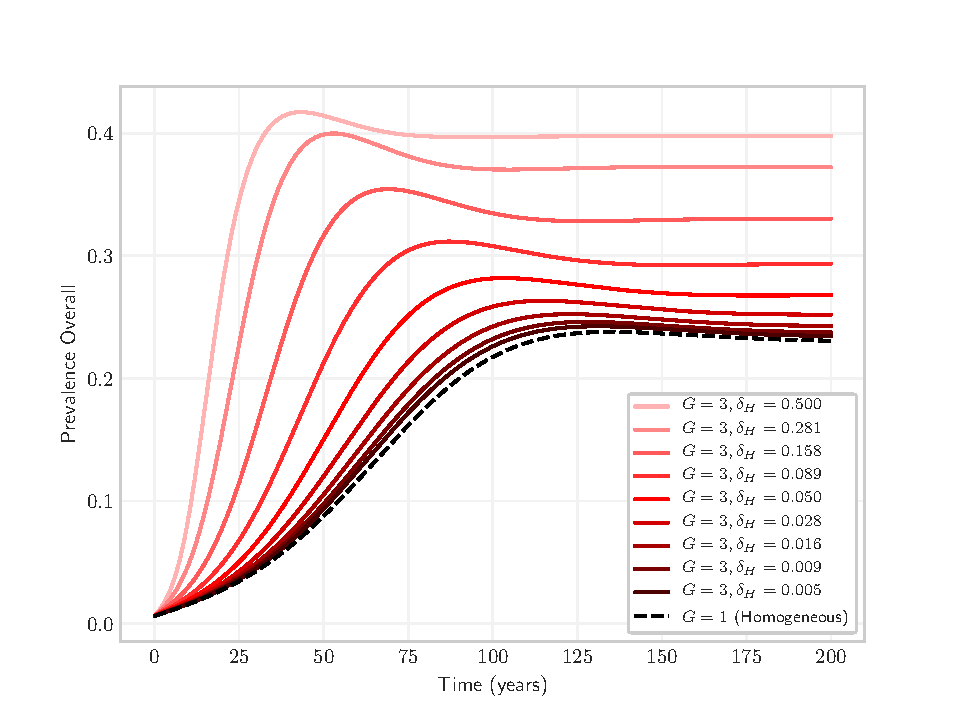
\includegraphics[width=0.6\linewidth]{hetero-converge}
  \caption{Overall prevalence predicted by a heterogeneous system
    for a range of high turnover rates.
    Note how the heterogeneous model ($G = 3$) converges on a homogeneous model ($G = 1$)
    with very high turnover rates.
    Compared to the Base model,
    transmission probability is increased to $\beta = [TBD]$
    in order to yield non-zero equilibrium prevalence in the homogeneous model.}
  \label{fig:hetero-converge}
\end{figure}
% ==================================================================================================
\subsection{Equilibrium Prevalence Before and After Model Calibration}
\begin{figure}[H]
  \centering
  \begin{subfigure}{0.45\linewidth}
    \centering
    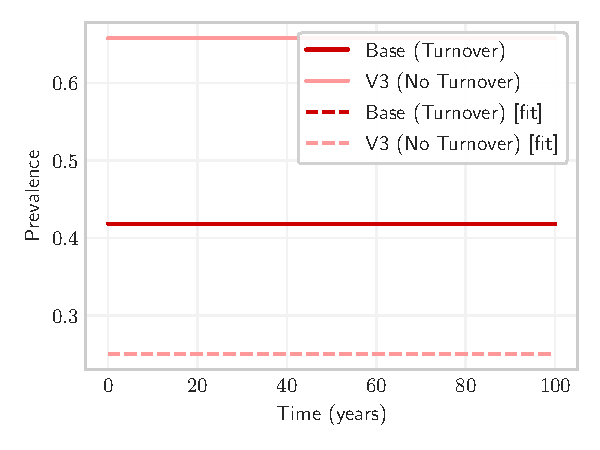
\includegraphics[width=\linewidth]{tpaf-prevalence-high}
    \caption{High risk}
    \label{fig:tpaf-prevalence-high}
  \end{subfigure}
  \begin{subfigure}{0.45\linewidth}
    \centering
    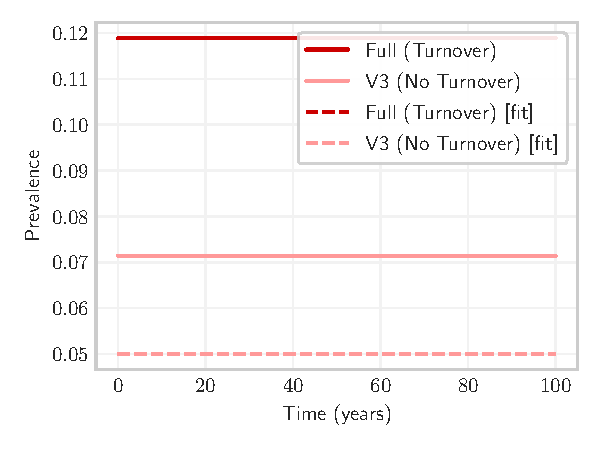
\includegraphics[width=\linewidth]{tpaf-prevalence-low}
    \caption{Low risk}
    \label{fig:tpaf-prevalence-low}
  \end{subfigure}
  \caption{Equilibrium prevalence among high and low risk groups
    with and without turnover,
    and with and without fitted $C_i$ to group-specific prevalence.}
  \label{fig:tpaf-prevalence}
\end{figure}
%% ==================================================================================================
%\subsection{Influence of Turnover}
%\newcommand{\idxiter}{%
%  0.1/Overall/all,
%  0.1/High risk/high,
%  0.1/Low risk/low,
%  0.2/Overall/all,
%  0.2/High risk/high,
%  0.2/Low risk/low}
%\begin{figure}[H]
%  \centering
%  \foreach \tx/\cap/\idx in \idxiter{
%    \begin{subfigure}{0.3\linewidth}
%      \centering
%      \includegraphics[width=\linewidth]{{turnover-prevalence-\idx-tau=\tx}.pdf}
%      \caption{\cap; $\tau = \tx$}
%    \end{subfigure}
%  }
%  \caption{Comparison of projected prevalence with and without risk group turnover,
%    under two different treatment rates $\tau$,
%    and one infected individual in each group at $t=0$.}
%  \label{fig:app-compare-turnover-prevalence}
%\end{figure}
%\begin{figure}[H]
%  \centering
%  \foreach \tx/\cap/\idx in \idxiter{
%    \begin{subfigure}{0.3\linewidth}
%      \centering
%      \includegraphics[width=\linewidth]{{turnover-incidence-\idx-tau=\tx}.pdf}
%      \caption{\cap; $\tau = \tx$}
%    \end{subfigure}
%  }
%  \caption{Comparison of projected incidence with and without risk group turnover,
%    under two different treatment rates $\tau$,
%    and one infected individual in each group at $t=0$.}
%  \label{fig:app-compare-turnover-incidence}
%\end{figure}
%\begin{figure}[H]
%  \centering
%  \foreach \tx/\cap/\idx in \idxiter{
%    \begin{subfigure}{0.3\linewidth}
%      \centering
%      \includegraphics[width=\linewidth]{{turnover-incidence-\idx-tau=\tx-p0e}.pdf}
%      \caption{\cap; $\tau = \tx$}
%    \end{subfigure}
%  }
%  \caption{Comparison of projected incidence with and without risk group turnover,
%    under two different treatment rates $\tau$,
%    and prevalence equal across groups at $t=0$.
%    Initial incidence is equal with and without turnover in all plots,
%    unlike Figure~\ref{fig:app-compare-turnover-incidence-p0e}.}
%  \label{fig:app-compare-turnover-incidence-p0e}
%\end{figure}
% ==================================================================================================
\subsection{Turnover of Infected Individuals}\label{aa:tinf}
\begin{figure}[H]
  \centering
  \includegraphics[width=0.6\linewidth]{{2d-tip-all-tau=0.1}.pdf}
  \caption{Proportion of new infections among each risk group
    which represent turnover of infected individuals
    versus infection of individuals in the risk group ($\tau = 0.1$).
    At high levels of turnover, an notable proportion of prevalence
    in all risk groups can be attributed to turnover of infected individuals
    from other risk groups.}
  \label{fig:new-inf-L}
\end{figure}